\chapter{Базовые понятия теории вероятностей}\label{ch:prob}
\todo[inline, author= Nozik, color = green]{Эту главу надо еще причесать как по порядку материала, так и по связности}
\disclaimer{
    Этот раздел рекомендуется для прочтения студентам, в программу которых на младших курсах не входит теория вероятностей. 
}

Определение понятия вероятности является сложной задачей без однозначно правильного решения. В зависимости от области применения, могут применяться различные, во многих случаях взаимоисключающие определения. При этом большинство определений приводят к одним и тем же практическим выводам, поэтому с прикладной точки зрения не так важно, какое из них выбрать. 

\section{Определение случайной величины}
\disclaimer{
    Конкретное определение вероятности не является существенным для практических применений, поэтому всем, кому не интересна идейная составляющая вопроса рекомендуется пропустить этот раздел и пользоваться "наивным" определением, основанном на "здравом смысле".
}

Как это ни парадоксально, формальная теория вероятности и математическая статистика никак не определяют понятие вероятности. Все теоретические выводы основываются на том, что изучаемые величины (вероятности) удовлетворяют некоторым формальным правилам (например системе аксиом Колмогорова \todo{ссылка}), но никаким образом не определяют как эти величины получить. Со времен создания теории вероятности существует два лагеря статистиков, каждый из которых использует свое определение.

\paragraph{Частотная вероятность}

\todo[inline, color = red]{ TODO Частотная вероятность}

\paragraph{Субъективная вероятность}

\todo[inline, color = red]{ TODO Субъективная вероятность}

Для упрощения понимания материала а также сокращения многих доказательств, в данном пособии мы будем придерживаться следующих определений:

\emph{Случайной} будем называть величину, значение которой не может быть \emph{достоверно} определено экспериментатором с абсолютной точностью или значение которой меняется в каждом последующем опыте неконтролируемым образом. Согласно такому определению, любой результат любых измерений является случайным, поскольку осведомленность экспериментатора всегда чем-то ограничена.

\section{Распределения}

Для работы со случайными величинами необходимо понимать, что они не являются полностью произвольными, а подчиняются некоторым законам. Эти законы называются распределениями.

\emph{Распределением случайной величины} $x$ или \emph{функцией плотности вероятности} называют такую функцию $f(x)$, что вероятность для нее находиться в диапазоне от $x$ до $x+dx$ равна $p(x \in (x_0, x_0+dx)) = f(x_0) dx$. Очевидно, что такое определение годится только для численным величин и имеет ряд других ограничений, но в данном пособии мы ограничимся им. Более строгие определения можно почерпнуть из специальной литературы (\todo{ссылка}).

Важно отметить, что в работах по статистике, написанных математиками, распределением часто называют не саму функцию $f$, а ее интеграл $F(x_0) = \int_{x_0}{f(x)dx}$, который можно определить, не используя бесконечно малые. Такую функцию физики называют \emph{интегральным распределением}.

Обозначим через $P\!\left(\left|\Delta x\right|<\delta\right)$ вероятность
(долю случаев) того, что отклонение от среднего $\Delta x=x-x_{0}$
составит величину, не превосходящую по модулю значение $\delta$:
\[
P\left(\left|\Delta x\right|<\delta\right)=\int\limits _{x_{0}-\delta}^{x_{0}+\delta}w\!\left(x\right)dx.
\]
Величину $P$ называют \emph{доверительной вероятностью} для \emph{доверительного
интервала} $\left|x-x_{0}\right|\le\delta$. 

Согласно определению вероятности, сумма вероятностей для всех возможных случаев всегда равна единице. Как следствие интеграл распределения $f$ в бесконечных пределах также всегда должен быть равен единицы. Это называют условием нормировки.

\subsection{Гистограмма}

Для визуализации распределений удобно использовать специальный тип графика: \emph{Гистограмму}.
Область значений $x$, размещённую на оси абсцисс, разобьём на равные малые интервалы --- <<корзины>>
или <<бины>> (\emph{англ.} bins) некоторого
размера $h$. По оси ординат будет откладывать долю измерений $w$,
результаты которых попадают в соответствующую корзину. Например, если
$n_{k}$ измерений лежит в диапазоне $kh<x<(k+1)h$, $k$ ---
номер корзины, то на графике изобразим столбик шириной $h$ и высотой
$w_{k}=n_{k}/n$. В результате получим картину, подобную изображённой
на рис.~\ref{fig:normhist}. 
% Самые высокие столбики будут сосредоточены
% вблизи среднего $\overline{x}$; ширина гистограммы будет по порядку
% величины равна $\sigma$, а при отклонении от $\overline{x}$ на несколько
% $\sigma$ столбиков не будет совсем.

\begin{figure}
    \centering
    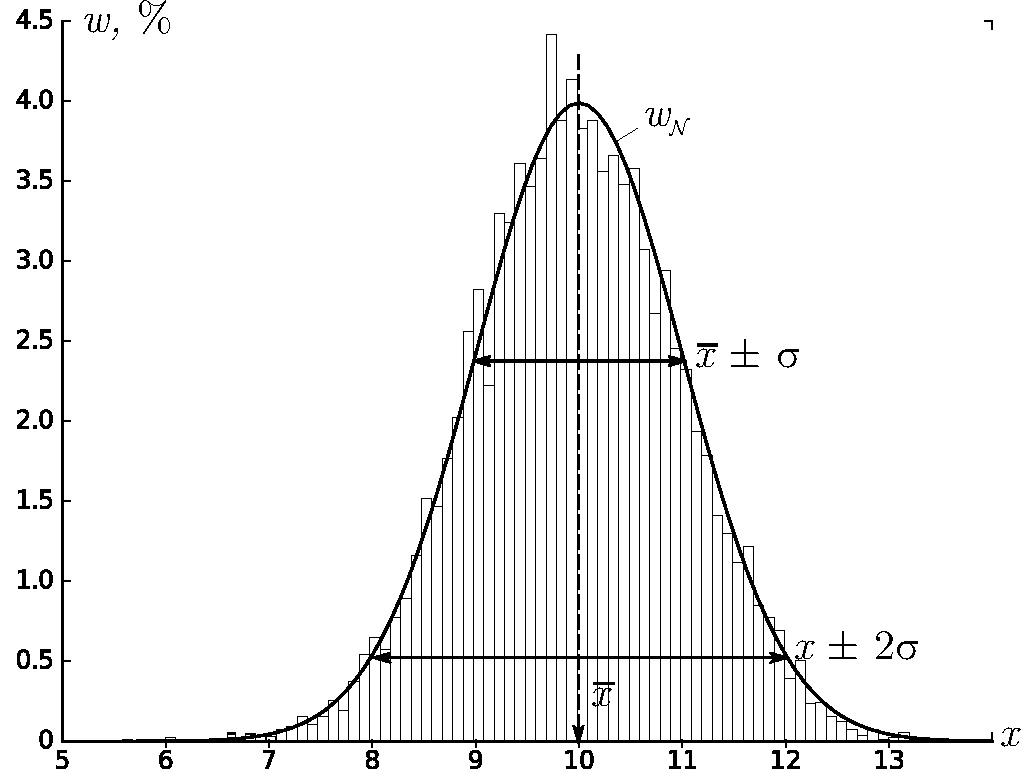
\includegraphics[width=7cm]{images/normhist.pdf}
    \label{fig:normhist}
    \caption{Пример гистограммы для нормального распределения ($\overline{x}=10$, $\sigma=1{,}0$, $h=0{,}1$, $n=10^{4}$)}
\end{figure}

% \disclaimer{
%     Этот раздел предназначен для  изучения методики проведения и анализа физического эксперимента на 2-3 курсах.
% }

% Предположим, что систематические погрешности малы и займёмся отдельно
% изучением случайных погрешностей. Пусть по результатам многократных
% измерений получен набор значений $\left\{ x_{i}\right\} $, вычислено
% их среднее (\ref{eq:average}) $\overline{x}$ и среднеквадратичное
% отклонение (\ref{eq:sigma}) $\sigma_{x}\approx s{}_{x}$. Можно надеяться,
% что измеряемая величина лежит в диапазоне
% \[
% x\in\left(\overline{x}-\sigma_{x};\,\overline{x}+\sigma_{x}\right).
% \]
% Какова вероятность $P$ того, что результат действительно находится
% в указанном интервале?

% Для ответа на этот вопрос необходимо знать \emph{вероятностный закон},
% которому подчиняется исследуемая величина. Казалось бы, для каждой
% случайной физической величины должен существовать свой особенный закон
% и общую теорию здесь построить невозможно. Это отчасти верно, но оказывается,
% что существует вполне \emph{универсальный} вероятностный закон, называемый
% \emph{нормальным}, которому подчиняются многие случайные величины.
% Рассмотрим его подробнее.

\section{Нормальное распределение}

Одним из наиболее примечательных результатов теории вероятностей является
так называемая \emph{центральная предельная теорема}, которая утверждает,
что сумма большого количества независимых случайных слагаемых, каждое
из которых вносит в эту сумму относительно малый вклад, подчиняется
универсальному закону, не зависимо от того, каким вероятностным законам
подчиняются её составляющие, --- так называемому \emph{нормальному
распределению} (или \emph{распределению Гаусса}). Эта теорема имеет
прямое отношение к физическим измерениям, поскольку зачастую случайные
погрешности складываются из множества случайных \emph{независимых}
факторов.

Доказательство теоремы довольно сложно и мы его не приводим. Остановимся
кратко на том, что такое нормальное распределение и его основных свойствах.

Плотность нормального распределения выражается следующей формулой:
\begin{equation}
    \label{eq:normal}
    \boxed{
        w_{\mathcal{N}}\!\left(x\right)=\frac{1}{\sqrt{2\pi}\sigma}e^{-\tfrac{(x-x_{0})^{2}}{2\sigma^{2}}}
    }.
\end{equation}
Здесь $x_{0}$ и $\sigma$
--- параметры нормального распределения: $x_{0}$ равно
среднему (и наиболее вероятному) значению $x$, a $\sigma$ ---
среднеквадратичному отклонению, вычисленным в пределе $n\to\infty$. 

Вероятность получить в результате эксперимента величину в диапазоне от $a$ до $b$ или вероятностное содержание интервала $(a,b)$ можно найти взяв соответствующий интеграл:
\begin{equation}
    P_{a\le x\le b}=\int\limits _{a}^{b}w\!\left(x\right)dx.\label{eq:P}
\end{equation}

Как видно из рис.~\ref{fig:normhist}, распределение представляет собой симметричный
<<колокол>>, положение вершины которого
соответствует среднему значению $\bar{x}$ (ввиду симметрии, оно же
совпадает с наиболее вероятным значением --- максимумом
функции $w_{\mathcal{N}}(x)$).

% \begin{figure}
%     \centering
%     \input{gauss.pdf_t}
%     \caption{Плотность нормального распределения}
% \end{figure}


При значительном отклонении $x$ от среднего величина $w_{\mathcal{N}}\!\left(x\right)$
быстро убывает. Это означает, что вероятность встретить отклонения,
существенно большие, чем $\sigma$, оказывается \emph{пренебрежимо
мала}. Ширина <<колокола>> по порядку величины
равна $\sigma$ --- она характеризует <<разброс>>
экспериментальных данных относительно среднего значения.

\note{
А именно, точки $x=\bar{x}\pm\sigma$ являются точками
перегиба графика $w\left(x\right)$ (в них вторая производная по $x$
обращается в нуль, $w''=0$), а их положение по высоте составляет
$w\!\left(\bar{x}\pm\sigma\right)/w(\bar{x})=e^{_{-1/2}}\approx0{,}61$
от высоты вершины.
}

Универсальный характер центральной предельной теоремы позволяет широко
применять на практике нормальное (гауссово) распределение для обработки
случайных погрешностей. Заметим, что на практике для \emph{приближённой
оценки} параметров нормального распределения случайной величины используются
\emph{выборочные} значения среднего и дисперсии: $x_{0}\approx\overline{x}$,
$s_{x}\approx\sigma_{x}$.

Для нормального распределения доверительные вероятности могут быть
легко найдены численно\footnote{Заметим, что интеграл $\int e^{-x^{2}/2}dx$, называемый \emph{интегралом
ошибок}, в элементарных функциях не выражается.}. Вероятность отклонения в пределах $\pm\sigma$ оказывается равна
\[
P\!\left(\left|\Delta x\right|<\sigma\right)\approx0{,}68,
\]
в пределах $\pm2\sigma$:
\[
P\!\left(\left|\Delta x\right|<2\sigma\right)\approx0{,}95,
\]
а в пределах $\pm3\sigma$:
\[
P\left(\left|\Delta x\right|<3\sigma\right)\approx0{,}9973.
\]
Таким образом, при большом числе измерений нормально распределённой
величины можно ожидать, например, что 68\% измерений попадут в интервал
$\left[\bar{x}-\sigma;\bar{x}+\sigma\right]$. При этом около 5\%
измерений выпадут за пределы $\left[\bar{x}-2\sigma;\bar{x}+2\sigma\right]$,
и лишь 0,27\% окажутся за пределами $\left[\bar{x}-3\sigma;\bar{x}+3\sigma\right]$.
Вероятность ещё больших отклонений очень быстро убывает\footnote{В сообщениях об открытии бозона Хиггса на Большом адронном коллайдере
говорилось о том, что исследователи ждали подтверждение результатов
с точностью <<5 сигма>>, ---
это означает, что они использовали доверительную вероятность $P\approx1-5{,}7\cdot10^{-7}=0{,}99999943$.
Такую точность можно назвать фантастической.}.

Полученные значения доверительных вероятностей используются при \emph{стандартной
записи результатов измерений}. В физических измерениях (в частности,
в учебной лаборатории), как правило, используется $P=0{,}68$, то
есть, запись 
\[
x=\bar{x}\pm\delta x
\]
означает, что измеренное значение лежит в диапазоне (доверительном
интервале) $x\in\left[\bar{x}-\delta x;\bar{x}+\delta x\right]$ с
вероятностью 68\%. Таким образом погрешность $\pm\delta x$ считается
равной одному среднеквадратичному отклонению: $\delta x=\sigma$.
В технических измерениях чаще используется $P=0{,}95$, то есть под
абсолютной погрешностью имеется в виду удвоенное среднеквадратичное
отклонение, $\delta x=2\sigma$. Во избежание разночтений доверительную
вероятность следует указывать отдельно.

\paragraph{Сравнение результатов измерений.}

Теперь мы можем дать количественный критерий для сравнения двух измеренных
величин или двух результатов измерения одной и той же величины.

Пусть величины $x_{1}$ и $x_{2}$ ($x_{1}\ne x_{2}$) измерены с
погрешностями $\sigma_{1}$ и $\sigma_{2}$ соответственно. 

Рассмотрим сперва случай, когда одна из величин известна с существенно
большей точностью: $\sigma_{2}\ll\sigma_{1}$ (например, $x_{1}$
--- результат, полученный студентом в лаборатории, $x_{2}$
--- справочное значение). Ясно, что если $\left|x_{1}-x_{2}\right|\gg\sigma_{1}$
то результаты заведомо не совпадают, а если $\left|x_{1}-x_{2}\right|\lesssim\sigma_{1}$,
то различия между ними можно объяснить случайным отклонением.

Поскольку $\sigma_{2}$ мало, значение $x_{2}$ можно принять за <<истинное>>
среднее и предположить, что погрешность измерения $x_{1}$ подчиняется
нормальному закону (со средним $x_{2}$ и дисперсией $\sigma_{1}^{2}$).
Тогда с помощью функции (\ref{eq:normal}) можно вычислить вероятность
$P\left(\left|x_{1}-x_{2}\right|\right)$ того, что отклонение $\left|x_{1}-x_{2}\right|$
возникло исключительно в силу случайных причин. Предварительно необходимо
договориться о том, какую вероятность отклонения следует считать \emph{значимой}.
Универсального значения здесь быть не может, поэтому приходится полагаться
на субъективный выбор конкретного исследователя. Часто в качестве
границы выбирают вероятность $P=0{,}05$, то есть результаты признаются
различными, если вероятность случайного отклонения меньше 5\%, и совпадающими
в противоположном случае. Как следует из свойств нормального распределения,
рассмотренных выше, такая вероятность соответствует отклонению на
$2\sigma$, то есть различие значимо, если 
\[
\left|x_{1}-x_{2}\right|>2\sigma_{1}.
\]

Пусть теперь погрешности двух измерений сравнимы по порядку величины,
$\sigma_{1}\sim\sigma_{2}$. В теории вероятностей показывается, что
линейная комбинация нормально распределённых величин также имеет нормальное
распределение. Следовательно, разность $x_{1}-x_{2}$ распределена
нормально с дисперсией $\sigma^{2}=\sigma_{1}^{2}+\sigma_{2}^{2}$
(см. также правила сложения погрешностей (\ref{eq:sigma_sum})). Тогда
для проверки гипотезы о том, что $x_{1}$ и $x_{2}$ являются измерениями
одной и той же величины, нужно вычислить, является ли значимым отклонение
$\left|x_{1}-x_{2}\right|$ от нуля.

\example{ 
Два студента получили
следующие значения для теплоты испарения некоторой жидкости: $x_{1}=40{,}3\pm0{,}2$
кДж/моль и $x_{2}=41{,}0\pm0{,}3$ кДж/моль, где погрешность соответствует
одному стандартному отклонению. Можно ли утверждать, что они исследовали
одну и ту же жидкость?

Имеем наблюдаемую разность $\left|x_{1}-x_{2}\right|=0{,}7$,
среднеквадратичное отклонение для разности $\sigma=\sqrt{0{,}2^{2}+0{,}3^{2}}=0{,}36$.
Их отношение $\frac{\left|x_{2}-x_{1}\right|}{\sigma}\approx2$. Из
свойств нормального распределения находим вероятность того, что измерялась
одна и та же величина, а различия в ответах возникли из-за случайных
ошибок: $P\approx5\%$. Ответ на вопрос, <<достаточно>>
ли мала или велика эта вероятность остаётся на усмотрение исследователя.
}

\note{
Изложенные здесь
соображения применимы, только если измеренное значение $x$ и его
стандартное отклонение $\sigma$ получены на основании достаточно
большой выборки $n\gg1$ (или заданы точно). Если приходится иметь
дело с небольшим количеством измерений ($n\lesssim10$), выборочные
средние и стандартные отклонения сами имеют довольно большую погрешность.
Тогда отклонения выборочных величин будут описываться не нормальным
распределением, а так называемым $t$-распределением Стъюдента. В
частности, в зависимости от значения $n$ интервал $\overline{x}\pm s_{x}$
будет соответствовать несколько меньшей доверительной вероятности,
чем $P=0{,}68$. Особенно резко различия проявляются при высоких уровнях
доверительных вероятностей $P\to1$. Подробнее об этом см. {[}?{]}.
}

\section{Распределение Пуассона}
\disclaimer{
    Распределение Пуассона применяется в случаях, когда имеет место измерения количества событий, произошедших за определенный интервал времени или в определенном объеме. Понимание этого распределения необходимо для студентов 5 семестра, изучающих основы физички частиц. Остальные студенты могут пропустить этот раздел.
}

\todo[inline, color = red]{TODO Пуассон}

\section{Независимые случайные величины. Корреляция}

Рассмотрим две физические величины $x$ и $y$. Величины называют
\emph{независимыми} если результат измерения одной из них никак не
влияет на результат измерения другой.

Обозначим отклонения от средних как $\Delta x=x-\overline{x}$ и $\Delta y=y-\overline{y}$.
Средние значения отклонений равны, очевидно, нулю: $\overline{\Delta x}=x-\overline{x}=0$,
$\overline{\Delta y}=0$. Из независимости величин $x$ и $y$ следует,
что среднее значение от произведения $\overline{\Delta x\cdot\Delta y}$
равно произведению средних $\overline{\Delta x}\cdot\overline{\Delta y}$
и, следовательно, равно нулю: 
\begin{equation}
\overline{\Delta x\cdot\Delta y}=\overline{\Delta x}\cdot\overline{\Delta y}=0.\label{eq:indep}
\end{equation}

Если $x$ и $y$ не являются независимыми, среднее значение произведения
их отклонений может быть использовано как количественная мера их зависимости.
Наиболее употребительной мерой зависимости двух случайных величин
является \emph{коэффициент линейной корреляции}:
\begin{equation}
r_{xy}=\frac{\overline{\Delta x\cdot\Delta y}}{\sigma_{x}\cdot\sigma_{y}}.\label{eq:pearson}
\end{equation}
Нетрудно проверить (с помощью неравенства Коши\textendash Буняковского),
что $-1\le r\le1$. В частности, для полностью независимых величин
коэффициент корреляции равен нулю, $r=0$, а для линейно зависимых
$y=kx+b$ нетрудно получить $r=1$ при $k>0$ и $r=-1$ при $k<0$.
Примеры промежуточных случаев представлены на рис. TODO.

Если коэффициент $r_{xy}$ близок к единице, говорят, что величины
\emph{коррелируют} между собой (от \emph{англ.} correlate ---
находиться в связи).

\paragraph{Отсутствие корреляции $\protect\not\Rightarrow$ независимость.}

Отметим, что (\ref{eq:indep}) --- необходимое,
но не достаточное условие независимости величин. На рис. TODO приведён
пример очевидно зависимых $x$ и $y$, для которых $r\approx0$.

\paragraph{Корреляция $\protect\not\Rightarrow$ причинность.}

Ещё одна типичная ошибка --- исходя из большого
коэффициента корреляции ($r\to1$) между двумя величинами сделать
вывод о функциональной (причинной) связи между $x$ и $y$. Рассмотрим
конкретный пример. Между током и напряжением на некотором резисторе
имеет место линейная зависимость $U=IR$, и коэффициент корреляции
$r_{UI}$ действительно равен единице. Однако \emph{обратное
в общем случае неверно}. Например, ток в резисторе коррелирует
с его температурой $T$, $r_{IT}\to1$ (больше ток --- больше
тепловыделение по закону Джоуля\textendash Ленца), однако ясно, что
нагрев резистора извне не приведёт к повышению тока в нём (скорее
наоборот, так как сопротивление металлов с температурой растёт). Ошибка
отождествления корреляции и причинности особенно характерна при исследовании
сложных многофакторных систем, например, в медицине, социологии и
т.п.

\section{Дисперсия суммы}

Пусть измеряемая величина $z=x+y$ складывается из двух \emph{независимы}х
случайных слагаемых $x$ и $y$, для которых известны средние значения
$\overline{x}$ и $\overline{y}$, и их среднеквадратичные погрешности
$\sigma_{x}$ и $\sigma_{y}$. Непосредственно из определения (\ref{eq:average})
следует вполне очевидный результат, что среднее суммы равно сумме
средних: 
\[
\overline{z}=\overline{x}+\overline{y}.
\]

Найдём дисперсию $\sigma_{z}^{2}$. В силу независимости имеем
\[
\overline{\Delta z^{2}}=\overline{\Delta x^{2}}+\overline{\Delta y^{2}}+2\overline{\Delta x\cdot\Delta y}=\overline{\Delta x^{2}}+\overline{\Delta y^{2}},
\]
то есть:
\begin{equation}
\boxed{{\sigma_{x+y}=\sqrt{\sigma_{x}^{2}+\sigma_{y}^{2}}}}.\label{eq:sigma_sum}
\end{equation}
Таким образом, при сложении \emph{независимых }величин их погрешности
складываются среднеквадратичным образом.

Подчеркнём, что для справедливости соотношения (\ref{eq:sigma_sum})
величины $x$ и $y$ не обязаны быть нормально распределёнными ---
достаточно существования конечных значений их дисперсий (однако можно
показать, что если $x$ и $y$ распределены нормально, нормальным
будет и распределение их суммы).

\note{
Требование независимости
слагаемых является принципиальным. Например, положим $y=x$. Тогда
$z=2x$. Здесь $y$ и $x$, очевидно, зависят друг от друга. Используя
(\ref{eq:sigma_sum}), находим $\sigma_{2x}=\sqrt{2}\sigma_{x}$,
что, конечно, неверно --- непосредственно из определения
следует, что $\sigma_{2x}=2\sigma_{x}$.
}

Отдельно стоит обсудить математическую структуру формулы (\ref{eq:sigma_sum}).
Если если одна из погрешностей много больше другой, например, $\sigma_{x}\gg\sigma_{y}$,
то меньшей погрешностью можно пренебречь, $\sigma_{x+y}\approx\sigma_{x}$.
С другой стороны, если два источника погрешностей имеют один порядок
$\sigma_{x}\sim\sigma_{y}$, то и $\sigma_{x+y}\sim\sigma_{x}\sim\sigma_{y}$. 

Эти обстоятельства важны при планирования эксперимента: как правило,
величина, измеренная наименее точно, вносит наибольший вклад в погрешность
конечного результата. При этом, пока не устранены наиболее существенные
ошибок, бессмысленно гнаться за повышением точности измерения остальных
величин.

\example{
Пусть $\sigma_{y}=\sigma_{x}/3$,
тогда $\sigma_{z}=\sigma_{x}\sqrt{1+\frac{1}{9}}\approx1{,}05\sigma_{x}$,
то есть при различии двух погрешностей более, чем в 3 раза, поправка
к погрешности составляет менее 5\%, и уже нет особого смысла в учёте
меньшей погрешности: $\sigma_{z}\approx\sigma_{x}$. Это утверждение
касается сложения любых независимых источников погрешностей в эксперименте.
}

\section{Погрешность среднего и отдельного измерений\label{sec:average}}

Выборочное среднее арифметическое значение $\overline{x}$, найденное
по результатам $n$ измерений, само является случайной величиной.
Действительно, если поставить серию одинаковых опытов по $n$ измерений,
то в каждом опыте получится своё среднее значение, отличающееся от
предельного среднего $x_{0}$.

Вычислим среднеквадратичную погрешность среднего арифметического $\sigma_{\overline{x}}$.
Рассмотрим вспомогательную сумму $n$ слагаемых 
\[
Z=x_{1}+x_{2}+\ldots+x_{n}.
\]
Если $\left\{ x_{i}\right\} $ есть набор \emph{независимых} измерений
\emph{одной и той же} физической величины, то мы можем, применяя результат
(\ref{eq:sigma_sum}) предыдущего параграфа, записать
\[
\sigma_{Z}=\sqrt{\sigma_{x_{1}}^{2}+\sigma_{x_{2}}^{2}+\ldots+\sigma_{x_{n}}^{2}}=\sqrt{n}\sigma_{x},
\]
поскольку под корнем находится $n$ одинаковых слагаемых. Отсюда с
учётом $\overline{x}=Z/n$ получаем
\begin{equation}
\boxed{{\sigma_{\overline{x}}=\frac{\sigma_{x}}{\sqrt{n}}}}.\label{eq:sigma_avg}
\end{equation}

Таким образом, \emph{погрешность среднего значения $x$ по результатам
$n$ независимых измерений оказывается в $\sqrt{n}$ раз меньше погрешности
отдельного измерения}. Это один из важнейших результатов, позволяющий
уменьшать случайные погрешности эксперимента за счёт многократного
повторения измерений.

Подчеркнём отличия между $\sigma_{x}$ и $\sigma_{\overline{x}}$:

величина $\sigma_{x}$ --- \emph{погрешность отдельного
измерения} --- является характеристикой разброса значений
в совокупности измерений $\left\{ x_{i}\right\} $, $i=1..n$. При
нормальном законе распределения примерно 68\% измерений попадают в
интервал $\overline{x}\pm\sigma_{x}$;

величина $\sigma_{\overline{x}}$ --- \emph{погрешность
среднего} --- характеризует точность, с которой определено
среднее значение измеряемой физической величины $\overline{x}$ относительно
предельного (<<истинного>>) среднего $x_{0}$;
при этом с доверительной вероятностью $P=68\%$ искомая величина $x_{0}$
лежит в интервале $\overline{x}-\sigma_{\overline{x}}<x_{0}<\overline{x}+\sigma_{\overline{x}}$.



% \section{Погрешность погрешности}
% \todo[inline, author = Nozik]{Вот это материал повышенной сложности. Не уверен, что он вообще нужен и уж точно не в середине главы}
% \todo[inline,author = ppv]{Сложности тут особой не вижу, но материал действительно побочный. Но полезный -- ведь это обоснование того, как нужно округлять погрешность.}

% С какой точностью можно вычислить величину $\sigma$ по ограниченному
% количеству $n$ измерений? Оценим среднеквадратичное отклонения от
% своего среднего значения для величины $s$, вычисляемой по формуле
% (\ref{eq:sigma_straight}). Её квадрат $s^{2}$, как нетрудно видеть,
% состоит из $n$ примерно одинаковых слагаемых (обозначим их как $\xi_{i}=\left(x_{i}-\overline{x}\right)^{2}$):
% \[
% s^{2}=\frac{1}{n-1}\sum_{i}\xi_{i}.
% \]
% Тогда, повторяя рассуждения п. \ref{subsec:average}, приходим к выводу,
% что погрешность вычисления $s^{2}$ пропорциональна корню из числа
% входящих в неё слагаемых (точнее, нужно использовать число \emph{независимых}
% слагаемых, равное $n-1$, как показано выше):
% \[
% \sigma_{s^{2}}\approx\sqrt{n}\cdot\frac{\sigma_{\xi}}{n-1}\approx
% \frac{\sigma_{\xi}}{\sqrt{n-1}}.
% \]
% С учётом того, что $\overline{\xi}\approx s^{2}\approx\sigma_{x}^{2}$,
% величину $\sigma_{\xi}=\sqrt{\overline{\left(\xi-\overline{\xi}\right)^{2}}}$
% можно по порядку величины оценить как $\sigma_{\xi}\sim\overline{\xi}\sim\sigma_{x}^{2}$;
% точный расчёт с использованием распределения Гаусса (\ref{eq:normal})
% даёт $\sigma_{\xi}=\sqrt{2}\sigma_{x}\approx\sqrt{2}s.$ Наконец,
% из соотношения $\sigma_{s^{2}}=2s\sigma_{s}$ (см. формулу (\ref{eq:sxy})
% ниже), окончательно получаем
% \begin{equation}
% \sigma_{s}=\frac{s}{\sqrt{2\left(n-1\right)}}.\label{eq:sigma_sigma}
% \end{equation}
% Более подробный и аккуратный вывод можно найти, например в {[}?{]}.

% Главный вывод, который можно сделать на основании результата (\ref{eq:sigma_sigma})
% --- ошибка вычисления стандартного отклонения, как правило,
% довольно велика. Например, при $n=6$ её относительная величина составляет
% $\approx$30\%, и даже при $n=50$ она уменьшается лишь до $10\%$.
% По этой причине величину погрешности имеет смысл \emph{округлять до
% 1\textendash 2 значащих цифр} (см. также п.~\ref{subsec:round}).

\section{Результирующая погрешность опыта}

Пусть для некоторого результата измерения известна оценка его максимальной
систематической погрешности $\Delta_{\text{сист}}$ и случайная среднеквадратичная
погрешность $\sigma_{\text{случ}}$. Какова <<полная>>
погрешность измерения?

Предположим для простоты, что измеряемая величина \emph{в принципе}
может быть определена сколь угодно точно, так что можно говорить о
некотором её <<истинном>> значении $x_{0}$
(иными словами, погрешность результата связана в основном именно с
процессом измерения). Назовём \emph{полной погрешностью} измерения
среднеквадратичное значения отклонения от результата измерения от
<<истинного>> $x_{0}$: 
\[
\sigma_{\text{полн}}^{2}=\overline{\left(x-x_{0}\right)^{2}}.
\]
Отклонение $x-x_{0}$ можно представить как сумму постоянной (но,
вообще говоря, неизвестной) систематической составляющей $\delta x_{\text{сист}}=\mathrm{const}$
и случайной добавки: $x-x_{0}=\delta x_{\text{сист}}+\delta x_{\text{случ}}$.
Причём среднее значение случайной составляющей равно нулю: $\overline{\delta x_{\text{случ}}}=0$.
В таком случае находим
\begin{equation}
\sigma_{\text{полн}}^{2}=\overline{\delta x_{\text{сист}}^{2}}+\overline{\delta x_{\text{случ}}^{2}}\le\Delta_{\text{сист}}^{2}+\sigma_{\text{случ}}^{2}.\label{eq:syst_full}
\end{equation}
Таким образом, для получения \emph{максимального} значения полной
погрешности некоторого измерения нужно среднеквадратично сложить максимальную
систематическую и случайную погрешности.

Если измерения проводятся многократно, то согласно (\ref{eq:sigma_avg})
случайная составляющая погрешности может быть уменьшена, а систематическая
составляющая при этом остаётся неизменной:
\[
\sigma_{\text{полн}}^{2}\le\Delta_{\text{сист}}^{2}+\frac{\sigma_{x}^{2}}{n}.
\]

Отсюда следует важное практическое правило (см. также обсуждение погрешности
суммы п. \ref{subsec:sum}): если случайная погрешность измерений
в 2\textendash 3 раза меньше предполагаемой систематической, то \emph{нет
смысла проводить многократные измерения} в попытке уменьшить погрешность
всего эксперимента. В такой ситуации измерения достаточно повторить
3\textendash 4 раза --- чтобы убедиться в повторяемости
результата, исключить промахи и проверить, что случайная ошибка действительно
мала. В противном случае повторение измерений может иметь смысл до
тех пор, пока погрешность среднего $\sigma_{\overline{x}}=\frac{\sigma_{x}}{\sqrt{n}}$
не станет существенно меньше систематической.

\note{
Поскольку конкретная
величина систематической погрешности, как правило, не известна, её
можно в некотором смысле рассматривать наравне со случайной ---
предположить, что её величина была определена по некоторому случайному
закону перед началом измерений (например, при изготовлении линейки
на заводе произошло некоторое случайное искажение шкалы). При такой
трактовке формулу (\ref{eq:syst_full}) можно рассматривать просто
как частный случай формулы сложения погрешностей независимых величин
(\ref{eq:sigma_sum}).\par

Подчеркнем, что вероятностный закон, которому подчиняется
систематическая ошибка, зачастую неизвестен. Поэтому неизвестно и
распределение итогового результата. Из этого, в частности, следует,
что мы не может приписать интервалу $x\pm\Delta_{\text{сист}}$ какую-либо
определённую доверительную вероятность --- она равна 0,68
только если систематическая ошибка имеет нормальное распределение.
Можно, конечно, \emph{предположить},
--- и так часто делают --- что, к примеру, ошибки
при изготовлении линеек на заводе имеют гауссов характер. Также часто
предполагают, что систематическая ошибка имеет \emph{равномерное}
распределение (то есть <<истинное>> значение может с равной вероятностью 
принять любое значение в пределах интервала $\pm\Delta_{\text{сист}}$). 
Строго говоря, для этих предположений нет достаточных оснований.\par
}%\footnotesize

\example{
В результате измерения диаметра проволоки микрометрическим винтом,
имеющим цену деления $h=0,01$ мм, получен следующий набор из $n=8$ значений:\par
\begin{tabular}{|c|c|c|c|c|c|c|c|c|}
\hline 
{\footnotesize{}$d$, мм} & {\footnotesize{}0,39} & {\footnotesize{}0,38} & {\footnotesize{}0,39} & {\footnotesize{}0,37} & {\footnotesize{}0,40} & {\footnotesize{}0,39} & {\footnotesize{}0,38} & {\footnotesize{}0,39}\tabularnewline
\hline 
\end{tabular}\par
Вычисляем среднее значение: $\overline{d}\approx386{,}3$~мкм.
Среднеквадратичное отклонение вычисляем по формуле (\ref{eq:sigma_straight}):
$\sigma_{d}\approx9{,}2$~мкм. Случайная погрешность среднего согласно
(\ref{eq:sigma_avg}): $\sigma_{\overline{d}}=\frac{\sigma_{d}}{\sqrt{8}}\approx3{,}2$
мкм. Все результаты лежат в пределах $\pm2\sigma_{d}$, поэтому нет
причин сомневаться в нормальности распределения. Максимальную погрешность
микрометра оценим как половину цены деления, $\Delta=\frac{h}{2}=5$~мкм.
Результирующая полная погрешность $\sigma\le\sqrt{\Delta^{2}+\frac{\sigma_{d}^{2}}{8}}\approx6{,}0$~мкм.
Видно, что $\sigma\approx\Delta$ и проводить дополнительные измерения
особого смысла нет. Окончательно результат измерений может быть представлен
в виде (см. также \emph{правила округления}
результатов измерений в п.~\ref{subsec:round})
\[
d=386\pm6\;\text{мкм},\qquad\varepsilon_{d}=1{,}5\%.
\]

Заметим, что поскольку случайная погрешность и погрешность
прибора здесь имеют один порядок величины, наблюдаемый случайный разброс
данных может быть связан как с неоднородностью сечения проволоки,
так и с дефектами микрометра (например, с неровностями зажимов, люфтом
винта, сухим трением, деформацией проволоки под действием микрометра
и т.\,п.). Для ответа на вопрос, что именно вызвало разброс, требуются
дополнительные исследования, желательно с использование более точных
приборов.\par
}%\footnotesize

\example{
Измерение скорости
полёта пули было осуществлено с погрешностью $\delta v=\pm1$ м/c.
Результаты измерений для $n=6$ выстрелов представлены в таблице:\par
\begin{tabular}{|c|c|c|c|c|c|c|}
\hline 
{\footnotesize{}$v$, м/с} & {\footnotesize{}146} & {\footnotesize{}170} & {\footnotesize{}160} & {\footnotesize{}181} & {\footnotesize{}147} & {\footnotesize{}168}\tabularnewline
\hline 
\end{tabular}\par
Усреднённый результат $\overline{v}=162{,}0\;\text{м/с}$,
среднеквадратичное отклонение $\sigma_{v}=13{,}8\;\text{м/c}$, случайная
ошибка для средней скорости $\sigma_{\bar{v}}=\sigma_{v}/\sqrt{6}=5{,}6\;\text{м/с}$.
Поскольку разброс экспериментальных данных существенно превышает погрешность
каждого измерения, $\sigma_{v}\gg\delta v$, он почти наверняка связан
с реальным различием скоростей пули в разных выстрелах, а не с ошибками
измерений. В качестве результата эксперимента представляют интерес
как среднее значение скоростей $\overline{v}=162\pm6\;\text{м/с}$
($\varepsilon\approx4\%$), так и значение $\sigma_{v}\approx14\;\text{м/с}$,
характеризующее разброс значений скоростей от выстрела к выстрелу.
Малая инструментальная погрешность в принципе позволяет более точно
измерить среднее и дисперсию, и исследовать закон распределения выстрелов
по скоростям более детально --- для этого требуется набрать
б\'{о}льшую статистику по выстрелам.\par
}%\footnotesize

\example{
Измерение скорости
полёта пули было осуществлено с погрешностью $\delta v=10$ м/c. Результаты
измерений для $n=6$ выстрелов представлены в таблице:\par
\begin{tabular}{|c|c|c|c|c|c|c|}
\hline 
{\footnotesize{}$v$, м/с} & {\footnotesize{}150} & {\footnotesize{}170} & {\footnotesize{}160} & {\footnotesize{}180} & {\footnotesize{}150} & {\footnotesize{}170}\tabularnewline
\hline 
\end{tabular}\par
Усреднённый результат $\overline{v}=163{,}3\;\text{м/с}$,
$\sigma_{v}=12{,}1\;\text{м/c}$, $\sigma_{\bar{v}}=5\;\text{м/с}$,
$\sigma_{\text{полн}}\approx11{,}2\;\text{м/с}$. Инструментальная
погрешность каждого измерения превышает разброс данных, поэтому в
этом опыте затруднительно сделать вывод о различии скоростей от выстрела
к выстрелу. Результат измерений скорости пули: $\overline{v}=163\pm11\;\text{м/с}$,
$\varepsilon\approx7\%$. Проводить дополнительные выстрелы при такой
большой инструментальной погрешности особого смысла нет ---
лучше поработать над точностью приборов и методикой измерений.\par
}%\footnotesize

\section{Обработка косвенных измерений\label{sec:kosv}}

\emph{Косвенными} называют измерения, полученные в результате расчётов,
использующих результаты \emph{прямых} (то есть <<непосредственных>>)
измерений физических величин. Сформулируем основные правила пересчёта
погрешностей при косвенных измерениях.

\subsection{Случай одной переменной}

Пусть в эксперименте измеряется величина $x$, а её <<наилучшее>>
(в некотором смысле) значение равно $x^{\star}$ и оно известно с
погрешностью $\sigma_{x}$. После чего с помощью известной функции
вычисляется величина $y=y\!\left(x\right)$.

В качестве <<наилучшего>> приближения для
$y$ используем значение функции при <<наилучшем>>
$x$:
\[
y^{\star}=y\!\left(x^{\star}\right).
\]

Найдём величину погрешности $\sigma_{y}$. Обозначая отклонение измеряемой
величины как $\Delta x=x-x^{\star}$, и пользуясь определением производной,
при условии, что функция $y\left(x\right)$ --- гладкая
вблизи $x\approx x^{\star}$, запишем 
\[
\Delta y\equiv y\left(x\right)-y\left(x^{\star}\right)\approx y'\cdot\Delta x,
\]
где $y'\equiv\frac{dy}{dx}$ --- производная, взятая в точке
$x^{\star}$. Возведём полученное в квадрат, проведём усреднение ($\sigma_{y}^{2}=\overline{\Delta y^{2}}$,
$\sigma_{x}^{2}=\overline{\Delta x^{2}}$), и затем снова извлечём
корень. В результате получим
\begin{equation}
\boxed{{\sigma_{y}=\left|\frac{dy}{dx}\right|\sigma_{x}.}}\label{eq:sxy}
\end{equation}

\example{
Для степенной функции
$y=Ax^{n}$ имеем $\sigma_{y}=nAx^{n-1}\sigma_{x}$, откуда 
\[
\frac{\sigma_{y}}{y}=n\frac{\sigma_{x}}{x},\qquad\text{или}\qquad\varepsilon_{y}=n\varepsilon_{x},
\]
то есть относительная погрешность степенной функции возрастает пропорционально
показателю степени $n$.\par
}%\footnotesize

\example{
$\varepsilon_{1/x}=\varepsilon_{x}$
--- при обращении величины сохраняется её относительная
погрешность.\par
}%\footnotesize

\note{ 
\textbf{Упражнение.} Найдите погрешность
логарифма $y=\ln x$, если известны~$x$ и~$\sigma_{x}$.\par
}%\footnotesize

\note{ 
\textbf{Упражнение.} Найдите погрешность
показательной функции $y=a^{x}$, если известны~$x$ и~$\sigma_{x}$.
Коэффициент $a$ задан точно.\par
}%\footnotesize

\subsection{Случай многих переменных}

Пусть величина $u$ вычисляется по измеренным значениям нескольких
различных \emph{независимых} физических величин $x$, $y$, $\ldots$
на основе известного закона $u=f\!\left(x,y,\ldots\right)$. В качестве
наилучшего значения можно по-прежнему взять значение функции $f$
при наилучших значениях измеряемых параметров:
\[
u^{\star}=f\!\left(x^{\star},y^{\star},\ldots\right).
\]

Для нахождения погрешности $\sigma_{u}$ воспользуемся свойством,
известным из математического анализа, --- малые приращения
функции многих переменных складываются линейно, то есть справедлив
\emph{принцип суперпозиции} малых приращений:
\[
\Delta u\approx f'_{x}\cdot\Delta x+f'_{y}\cdot\Delta y+\ldots,
\]
где символом $f'_{x}\equiv\frac{\partial f}{\partial x}$ обозначена
\emph{частная производная} функции $f$ по переменной $x$ ---
то есть обычная производная $f$ по $x$, взятая при условии, что
все остальные аргументы (кроме $x$) считаются постоянными параметрами.
Тогда пользуясь формулой для нахождения дисперсии суммы независимых
величин (\ref{eq:sigma_sum}), получим соотношение, позволяющее вычислять
погрешности косвенных измерений для произвольной функции $u=f\left(x,y,\ldots\right)$:
\begin{equation}
\boxed{\sigma_{u}^{2}=f_{x}^{\prime2}\,\sigma_{x}^{2}+f_{y}^{\prime2}\,\sigma_{y}^{2}+\ldots}\label{eq:sigma_general}
\end{equation}
Это и есть искомая общая формула пересчёта погрешностей при косвенных
измерениях.

Отметим, что формулы (\ref{eq:sxy}) и (\ref{eq:sigma_general}) применимы
только если относительные отклонения всех величин малы ($\varepsilon_{x},\varepsilon_{y},\ldots\ll1$),
а измерения проводятся вдали от особых точек функции $f$ (производные
$f_{x}'$, $f_{y}'$ $\ldots$ не должны обращаться в бесконечность).
Также подчеркнём, что все полученные здесь формулы справедливы только
для \emph{независимых} переменных $x$, $y$, $\ldots$

Остановимся на некоторых важных частных случаях формулы (\ref{eq:sigma_general}).

\paragraph{Погрешность суммы.}

Для суммы (или разности) $u=\sum\limits _{i=1}^{n}a_{i}x_{i}$ имеем
\begin{equation}
\sigma_{u}^{2}=\sum_{i=1}^{n}a_{i}^{2}\sigma_{x_{i}}^{2}.
\end{equation}


\paragraph{Погрешность степенной функции.}

Пусть $u=x^{\alpha}\cdot y^{\beta}\cdot\ldots$. Тогда нетрудно получить,
что
\[
\frac{\sigma_{u}^{2}}{u^{2}}=\alpha^{2}\frac{\sigma_{x}^{2}}{x^{2}}+\beta^{2}\frac{\sigma_{y}^{2}}{y^{2}}+\ldots
\]
или через относительные погрешности
\begin{equation}
\varepsilon_{u}^{2}=\alpha^{2}\varepsilon_{x}^{2}+\beta^{2}\varepsilon_{y}^{2}+\ldots\label{eq:espilon_power}
\end{equation}


\paragraph{Погрешность произведения и частного.}

Пусть $u=xy$ или $u=x/y$. Тогда в обоих случаях имеем
\begin{equation}
\varepsilon_{u}^{2}=\varepsilon_{x}^{2}+\varepsilon_{y}^{2},
\end{equation}
то есть при умножении или делении относительные погрешности складываются
квадратично.

{\footnotesize
\textbf{Пример.} Рассмотрим несколько
более сложный пример: нахождение угла по его тангенсу 
\[
u=\arctg\frac{y}{x}.
\]
В таком случае, пользуясь тем, что $\left(\arctg z\right)'=\frac{1}{1+z^{2}}$,
где $z=y/x$, и используя производную сложной функции, находим $u_{x}'=u_{z}'z'_{x}=-\frac{y}{x^{2}+y^{2}}$,
$u_{y}'=u'_{z}z'_{y}=\frac{x}{x^{2}+y^{2}}$, и наконец 
\[
\sigma_{u}^{2}=\frac{y^{2}\sigma_{x}^{2}+x^{2}\sigma_{y}^{2}}{\left(x^{2}+y^{2}\right)^{2}}.
\]
}%\footnotesize

{\footnotesize
\textbf{Упражнение.} Найти погрешность
вычисления гипотенузы $z=\sqrt{x^{2}+y^{2}}$ прямоугольного треугольника
по измеренным катетам $x$ и $y$.\par
}%\footnotesize

По итогам данного раздела можно дать следующие практические рекомендации.
\begin{itemize}
\item Как правило, нет смысла увеличивать точность измерения какой-то одной
величины, если другие величины, используемые в расчётах, остаются
измеренными относительно грубо --- всё равно итоговая погрешность
скорее всего будет определяться самым неточным измерением. Поэтому
все измерения имеет смысл проводить \emph{примерно с одной и той же
относительной погрешностью}. 
\item При этом, как следует из (\ref{eq:espilon_power}), особое внимание
следует уделять измерению величин, возводимых при расчётах в степени
с большими показателями. А при сложных функциональных зависимостях
имеет смысл детально проанализировать структуру формулы (\ref{eq:sigma_general}):
если вклад от некоторой величины в общую погрешность мал, нет смысла
гнаться за высокой точностью её измерения, и наоборот, точность некоторых
измерений может оказаться критически важной.
\item Следует избегать измерения малых величин как разности двух близких
значений (например, толщины стенки цилиндра как разности внутреннего
и внешнего радиусов): если $u=x-y$, то абсолютная погрешность $\sigma_{u}=\sqrt{\sigma_{x}^{2}+\sigma_{y}^{2}}$
меняется мало, однако относительная погрешность $\varepsilon_{u}=\frac{\sigma_{u}}{x-y}$
может оказаться неприемлемо большой, если $x\approx y$.
\end{itemize}